\section{Auswertung}
\label{sec:Auswertung}

\subsection{Temperaturmessung}
Der gemessene Offset beträgt am Anfang der Messreihe $U_{0,Anfang} = \SI{0,0075}{\milli\volt}$ und am Ende $U_{0,Ende} = \SI{0,0088}{\milli\volt}$
Der Mittelwert beträgt dementsprechend $U_0 = \SI{0.00815}{\milli\volt}$.
$\Delta U = U_i - U_0$ ist demnach die wahre Spannung.
Die Temperatur im Raum betrug in etwa $T_0 = \SI{297,6}{\kelvin}$
Im Folgenden sind die Messdaten für matt, schwarz, glänzend und weiß in jener Reihenfolge aufgeführt:
\\
(Tabelle 1-4)
\\
Im obrigen Diagramm wurden die Spannungen $\Delta U_i$ gegen die Differenz $T^4 - T_0^4$ aufgetragen.
Es wird ein linearer Zusammenhang der Form
\begin{equation}
  f(x) = mx + b
\end{equation}
erwartet.
Die Ausgleichsrechnung wird mit Hilfe der Gaußschen Methode der kleinsten Abweichungsquadrate durchgeführt.
Für die Steigung $m$ wird die Formel
\begin{equation}
  m = \frac{ n \sum_{i=1}^n x_i y_i - \sum_{i=1}^n x_i \sum_{i=1}^n y_i }{n\sum_{i=1}^n x_i^2 - ( \sum_{i=1}^n x_i )^2}
\end{equation}
verwendet. Dabei bezeichnet $n$ die Anzahl der Messungen, für $x_i$ und $y_i$ werden die jeweiligen Messwerte eingesetzt. Der Schnittpunkt mit der y-Achse wird durch
\begin{equation}
  b = \frac{ \sum_{i=1}^n x_i^2 \cdot \sum_{i=1}^n y_i - \sum_{i=1}^n x_i \cdot \sum_{i=1}^n x_i y_i}{n\sum_{i=1}^n x_i^2 - ( \sum_{i=1}^n x_i )^2}
\end{equation}

beschrieben.
Die Standardabweichung in y berechnet sich zu
\begin{equation}
  \sigma_y = \sqrt{ \frac {\sum_{i=1}^n (y_i-b-m \cdot x_i)}{n-2} }.
\end{equation}
Hieraus ergibt sich sofort
\begin{equation}
  \sigma_m = \sqrt{ \sigma_y^2 \frac{n}{n \sum_{i=1}^n x_i^2 - (\sum_{i=1}^n x)^2} }
\end{equation}
sowie
\begin{equation}
  \sigma_b = \sqrt{ \sigma_y^2 \frac{\sum_{i=1}^n x_i^2}{n \sum_{i=1}^n x_i^2 - (\sum_{i=1}^n x)^2} }
\end{equation}
für die Standardabweichungen in m und b.

\subsection{Abstandsmessung}


\begin{figure}
  \centering
  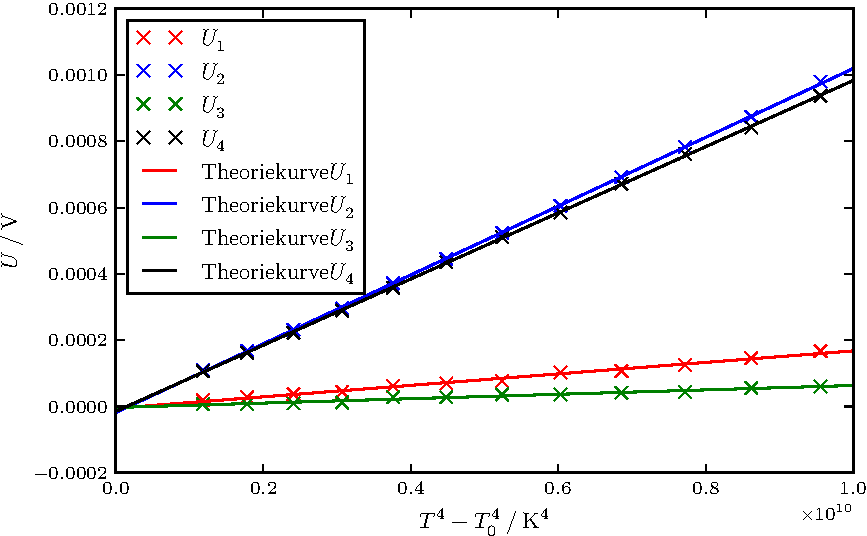
\includegraphics{plot.pdf}
  \caption{Plot.}
  \label{fig:plot}
\end{figure}
